\section{Linguaggi formali}
Per \textbf{linguaggio formale} intendiamo un insieme di stringhe composte da simboli di un alfabeto $\Sigma$, definito come un insieme non vuoto di
questi ultimi.\par
In particolare, un \textbf{simbolo} è un'entità primitiva astratta non definita formalmente, come lettere e cifre; una loro sequenza finita è detta
\textbf{stringa}, la quale avrà una \textbf{lunghezza} $|w|$ che indica il numero di occorrenze di simboli che la compongono, per esempio: \[
    abbba \implies |w| = 5
\]

\noindent In questi termini è necessario notare come l'ambito di questa materia sarà tradurre il calcolo delle funzioni in relazioni di insieme.
Esistono diversi tipi di linguaggi: \begin{itemize}
    \item \textbf{Linguaggio finito}: Composto da sole costanti, non richiede alcuna memoria e non ci sono input sconosciuti.
    \item \textbf{Linguaggio regolare}: Si traduce in una funzione lineare per la quale serve memoria, ma di quantità finita necessaria per calcolarla.
    \item \textbf{Linguaggio context free}: Non è conosciuta la quantità di memoria richiesta per calcolare la funzione, richiede una stack.
    \item \textbf{Linguaggio decidibile}: Funzione per la quale la stack non è sufficiente e si richiede ulteriore memoria a supporto.
\end{itemize}

%

\section{Automi a stati finiti}
Un \textbf{Automa a stati finiti} è il modello di un sistema avente input e un eventuale output a valori discreti. Il sistema può trovarsi in uno stato
all'interno di un loro insieme finito e ciò gli consente di tenere traccia della storia precedente, quindi di avere una memoria finita.\par
Questi modelli sono rappresentabili mediante una testina che legge un nastro di lunghezza illimitata contenente i simboli. In base allo stato corrente
$q$ e del simbolo letto $s_i$, la testina vedrà se spostarsi in un altro stato o meno, e leggerà il simbolo successivo. Alla terminazione della lettura,
in base allo stato raggiunto, l'automa fornirà un risultato di accettazione o rifiuto della stringa letta.\par
Il comportamento degli automi è definito univocamente con una tabella chiamata \textbf{matrice di transizione}, e sono rappresentati con il seguente
grafo: \begin{figure}[h]
	\centering
	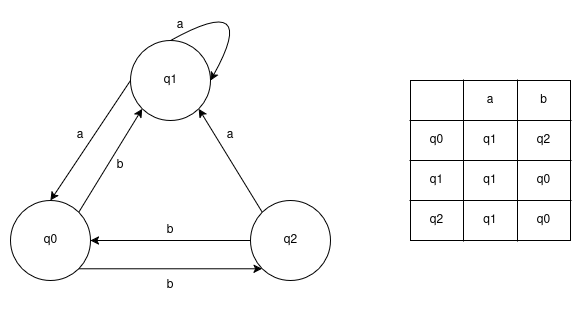
\includegraphics[width=0.8\linewidth]{Images/DFA_example.png}
	\caption{Esempio di automa a stati finiti}
\end{figure}

\subsection{Automi a stati finiti deterministici}
Gli Automi a stati finiti deterministici (DFA) sono una sottoinsieme di automi, definiti come una quintupla $M = (Q, \Sigma, \delta, q_0, F)$, i cui
elementi sono: \begin{itemize}
    \item $Q$: Insieme finito degli stati.
    \item $\Sigma$: Alfabeto dei simboli che l'automa può riconoscere.
    \item $\delta:Q\times\Sigma \to Q$: Funzione di transizione degli stati, la quale, data una coppia (stato, simbolo), ritorna lo stato successivo.
    \item $q_0$: Stato iniziale dell'automa.
    \item $F\subseteq Q$: Insieme degli stati finali che descrive i risultati accettabili ottenibili dall'automa.
\end{itemize}

\noindent Dalla funzione di transizione $\delta$ si ottiene anche in modo univoco quella che descrive lo stato raggiunto dopo aver letto una sequenza di
simboli $\hat{\delta}:Q \times \Sigma^* \to Q$ nel seguente modo: \[ \begin{cases}
		\hat{\delta}(q,\epsilon) = q\\
		\hat{\delta}(q, \omega a) = \delta(\hat{\delta}(q,w)a)
\end{cases} \]

\noindent Questa funzione è detta \textbf{chiusura transitiva di} $\delta$; nel primo caso l'automa non legge nulla, mentre nella seconda espressione si
indica che ha letto una sequenza di caratteri e un nuovo simbolo annotato con $a$.\par
Tuttavia, menzionando la possibilità di ritornare un risultato di non accettazione, ne consegue che esistano dei simboli (e di conseguenza, linguaggi),
non riconoscibili dall'automa. Questa caratteristica è il discriminante che consente di definire i \textbf{linguaggi regolari}: tali se e solo se esiste
un automa a stati finiti deterministico $M$ che lo riconosce. Vengono definiti come: \[
    L_m = \{\sigma\in \Sigma^* | \hat{\delta}(q_0, \sigma)\in F\}
\]

\noindent L'insieme dei linguaggi caratterizzati dall'essere riconosciuti da un DFA è detto \textbf{insieme dei linguaggi regolari}, e per dimostrare
che un linguaggio $L$ gli appartiene è necessario fornire un DFA capace di riconoscerlo correttamente. Per esempio, supposto l'alfabeto $\Sigma =
\{a, b\}$ e il linguaggio $\emptyset$, viene generato il seguente automa: \[
    M_{\emptyset} = \left<\{q_0\}, \{a, b\}, \delta, q_0, \emptyset\right>
\]

\noindent Affermando che $\emptyset = L_m$, otteniamo: \[
    L_m = \{\sigma\in Sigma^* | \hat{\delta}(q_0, \sigma)\in F\}
\]

\noindent Semanticamente parlando, notiamo che è impossibile che l'automa si muova se non legge niente, infatti l'espressione $\hat{\delta}(q_0, \sigma)
\in F$ è sempre falsa, definendo il corretto comportamento dell'automa quando non accade niente e provando che $\emptyset$ è un linguaggio regolare.
Supponiamo ora un linguaggio di stringhe che contengono almeno due '1' sull'alfabeto $\Sigma = \{0,1\}$, quindi: \[
    L = \{x\in \Sigma^* | x \text{contiene due '1'}\}
\]

\noindent Costruiamo un automa $M$ a tre stati definito dalla seguente matrice di transizione: \begin{table}[h]
	\centering
	\begin{tabular}{c|c|c|}
		& $i=0$ & $i=1$\\
		\hline
		$q_0$ & $q_0$ & $q_1$\\
		\hline
		$q_1$ & $q_1$ & $q_2$\\
		\hline
		$q_2$ & $q_2$ & $q_2$\\
		\hline
	\end{tabular}
	\caption{Matrice di transizione}
\end{table}

\noindent Questo deve riconoscere il linguaggio, il quale deve essere $L = L(m)$, che è equivalente a dire $L \subseteq L(m) \land L(m) \subseteq L$,
ovvero tutto il linguaggio è riconosciuto da $M$ e il linguaggio riconosciuto da $M$ è contenuto in $L$. Dimostriamo le due tesi: \begin{itemize}
    \item $L \subseteq L(m) \iff \forall x\in \Sigma^{*}.x\in L \implies x\in L(m) \implies \hat{\delta}(q_0, x)\in F$\par
    Dunque per ogni stringa componibile con $\Sigma^*$ è necessario che si riesca ad arrivare a uno stato finale.
    \item $L(m) \subseteq L \iff x\in L(m) \implies x\in L$\par
    Ovvero la stringa del linguaggio formale deve essere anche contenuta in quello che si vuole dimostrare tale.
\end{itemize}

\noindent Notare che per la seconda dimostrazione, la prima tesi vale se e solo se si riesce ad arrivare a uno stato finale con la stringa $x$,
necessariamente contenuta in $L$. Poste queste basi per il linguaggio, possiamo procedere a dimostrare la regolarità di $L$ per induzione sulla
lunghezza di $x$, mostrando che: \[ \begin{cases}
    x\in L \implies \hat{\delta}(q_0, x)\in F\\
    x\notin L \implies \hat{\delta}(q_0, x)\notin F
\end{cases} \]

\paragraph{Passo base:} $|x| = 0 \iff x = \epsilon$\par
Bisogna prendere la più piccola lunghezza che garantisca sia stringhe in $L$ che stringhe ad esso non appartenenti. |x| = 2 è sufficiente. Procediamo a
dimostrare la base per ogni lunghezza fino a due: \begin{itemize}
    \item $|x| = 0$: \[
        \hat{\delta}(q_0, x) = \hat{\delta}(q_0, \epsilon) = q_0\notin F
    \]
    \item $|x| = 1$: \[ \begin{cases}
        x = 0\notin L &\implies \hat{\delta}(q_0, 0) = \delta(q_0, 0) = q_0\notin F\\
        x = 1\notin L &\implies \hat{\delta}(q_0, 1) = \delta(1_0, 1) = q_1\notin F
    \end{cases} \]
    \item $|x| = 2$: \[ \begin{cases}
        x = 00\notin L &\implies \hat{\delta}(q_0, x) = q_0\notin F\\
        x = 01\notin L &\implies \hat{\delta}(q_0, x) = q_1\notin F\\
        x = 10\notin L &\implies \hat{\delta}(q_0, x) = q_1\notin F\\
        x = 11\in L &\implies \hat{\delta}(q_0, x) = \delta(\hat{\delta}(q_0, 1), 1) = \delta(q_1, 1) = q_2\in F
    \end{cases} \]
\end{itemize}

\noindent Questa è la definizione formale della base, per cui si dice che ogni stringa di lunghezza uguale a 2 che non contiene due cifre '1' non è
accettata all'interno del linguaggio.

\paragraph{Passo induttivo:} Sempre in riferimento alla lunghezza della stringa, è necessario dimostrare che per $|z| = n+1$ valga la seguente ipotesi
induttiva: sia $n\in N$; $\forall x.|x|\leq n$: \[ \begin{cases}
    x\in L \implies \hat{\delta}(q_0, x)\in F\\
    x\notin L \implies \hat{\delta}(q_0, x)\notin F
\end{cases} \]

\noindent Con una lunghezza della stringa non ben definita, è possibile che si abbiano $x = x'0$ oppure $x = x'1$, dipendentemente da cosa l'automa
legge. Definiamo i casi: \begin{itemize}
    \item $x'\in L \implies x\in L$ per definizione, e per ipotesi induttiva porta allo stato finale: \[
        \hat{\delta}(q_0, x') = q_2
    \]
    \item Se $x'\notin L$ e $x = x'1$ l'automa ha letto almeno una cifra '1'. Bisogna leggere il seguente simbolo. Se $x'$ contiene '1', allora $x\in L$,
	altrimenti $x\notin L$.
    \item Se $x'\notin L$ e $x = x'0$ l'automa non ha ancora letto una cifra '1'; in questi termini non è possibile raggiungere uno stato finale, quindi
	varrà $x\notin L$ a prescindere dalla lettura di $x'0$ o $x'1$. Dunque: \[
        \hat{\delta}(q_0, x) = \delta(\hat{\delta}(q_0, x'), 0) \in \{q_0q_1\}\nsubseteq F
    \]
\end{itemize}

\subsection{Automi a stati finiti non deterministici}

%

\section{Linguaggi liberi da contesto, forme normali e automi a pila}

%

\section{Classificazione di Chomsky}